%%%%%%%%%%%%%%%%%%%%%%%%%%%%%%%%%%%%%%%%%%%%%%
%                insertmeeting
% 1) Title (something creative & funny?)
% 2) Date (MM/DD/YYYY)
% 3) Location (ex. Hagerty High School)
% 4) People/Committees Present 
% 5) Picture 
% 6) Start Time & Stop Time (ex. 12:30AM to 4:30PM)
%%%%%%%%%%%%%%%%%%%%%%%%%%%%%%%%%%%%%%%%%%%%%%
\insertmeeting 
	{Imaginative Implementations} 
	{01/11/22} 
	{Hagerty High School}
	{Annika, Anouska, Clayton, Falon, James, Jensen, Nathan, Ritam, Rose, Samantha, Lilly}
	{Images/RobotPics/robot.jpg}
	{2:30 - 4:30}
	
\hhscommittee{Software}
\noindent\hfil\rule{\textwidth}{.4pt}\hfil
\subsubsection*{Goals}
\begin{itemize}
    \item Begin to implement our derived tricycle kinematic equations into an extendible Kotlin class.   

\end{itemize} 

\noindent\hfil\rule{\textwidth}{.4pt}\hfil

\subsubsection*{Accomplishments}
After verifying that our tricycle kinematic equations were correct, we wanted to begin implementing it into our code. This was a monumental task, as it involved modifying existing localization systems while ensuring that they can still work with the pre-existing TRC event systems and Road Runner. But to simplify that task, we broke it down into smaller portions. Our first goal was to create classes similar to "TankDrive" and "TankKinematics" in the Road Runner library that would be able to hold the methods and data we will need for our tricycle drive. We started by using a template from the sample Tank Drive Kinematics provided by Road Runner. We took the localization calculations and inserted them where the tank kinematic equations were. This new file, "TricycleKinematics.kt" allowed us to continue localization the robot using our uncommon wheel encoder tracking. We would later use these functions in a class titled "TricycleDrive.kt" that represented the drivebase to use in Road Runner. It contained modified methods to update() the drive position using the new tricycle kinematics equations. Next, we have to test these methods in conjunction with Road Runner to find any errors. 
 

\begin{figure}[htp]
\centering
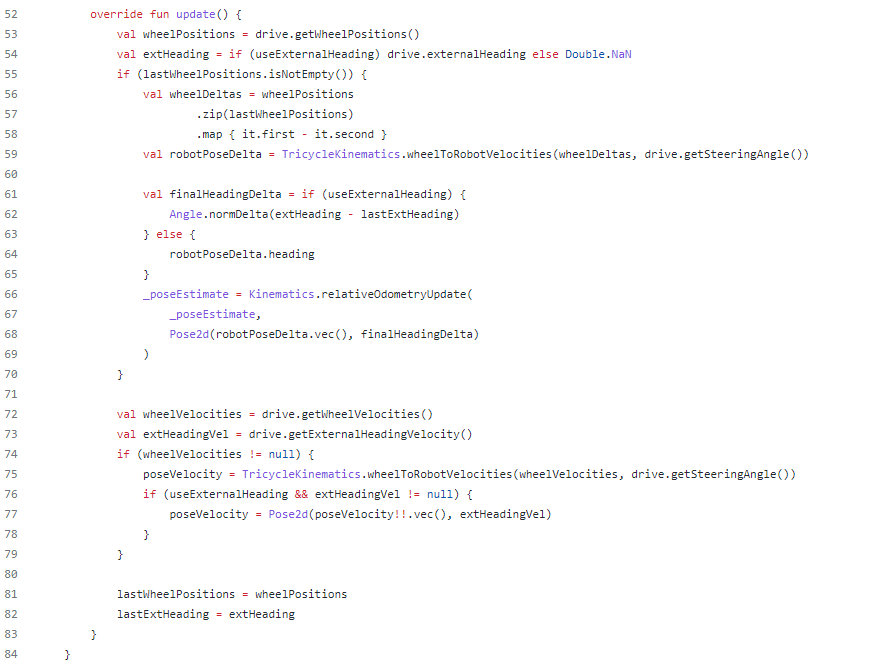
\includegraphics[width=0.95\textwidth, angle=0]{Meetings/January/01-11-22/1.13.22 tricyledrive.kt - James Hu.PNG}
\caption{Our update method, created based on samples provided by Road Runner}
\label{fig:011122_1}
\end{figure}

\begin{figure}[htp]
\centering
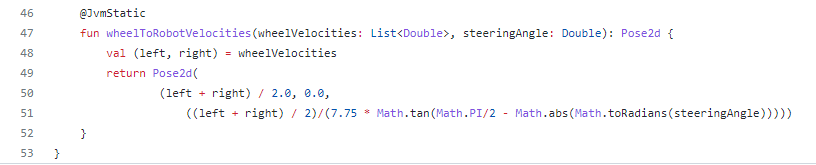
\includegraphics[width=0.95\textwidth, angle=0]{Meetings/January/01-11-22/1.13.22 tricyledrivekinematics.kt - James Hu.PNG}
\caption{Implementing the new kinematic equations into our code}
\label{fig:011122_2}
\end{figure}


\hhscommittee{Hardware}
\noindent\hfil\rule{\textwidth}{.4pt}\hfil
\subsubsection*{Goals}
\begin{itemize}
    \item Build sweeper intake 
	\item Test sweeper intake
  

\end{itemize} 

\noindent\hfil\rule{\textwidth}{.4pt}\hfil

\subsubsection*{Accomplishments}
With only a few days until the next meet, we came into the meeting today ready to build and test our newly designed sweeper intake. We started by gathering all of the parts including XL belts (with a 27:10 reduction for speed), the 3d printed base, the spinner part, and the laser cut sides, which we laser cut at the beginning of the meeting on our glowforge. Because we designed this intake to be easy to edit, putting it together was as simple as screwing in the side plates, attaching the servo, and adding the spinner. With the intake almost entirely built fairly quickly, we had plenty of time to test it out. One thing we still needed to decide upon was what material to use as the flaps. We started by testing with rubber strips we cut out of a sheet of rubber, which was our front runner for flap material. We found that the rubber performed pretty well and was definitely able to grab and hold blocks reliably. We did however think that the speed at which the intake could suck in blocks was less than we anticipated, so we tried testing with some stiffer materials, like surgical tubing. The surgical tubing, as expected, grabbed blocks much quicker and easier, but the stiffness of the tubing caused the spinner to get jammed occasionally. When testing on balls instead of blocks, the situation was even worse. The surgical tubing bound up more than half the time, damaging the servo by preventing it from moving. Deciding to switch back to the more reliable rubber flaps, we once again tested with balls checking more thoroughly to make sure we were not damaging the servo like the surgical tubing had. As we watched, we found a similar issue if the rubber strips were too long. Because of this, we cut the strips to a point where they could still grab the elements, but wouldn’t get jammed. No matter their length, the strips still put a small amount of strain on the servo when intaking balls, forcing us to the decision to go only for blocks if possible. Although this shouldn't be a significant hindrance at the meet, it is still less than optimal and a change we will have to try to make before the league championship. All in all, we are happy with how the intake turned out, and are planning on using it at the upcoming 4th meet (Figure \ref{fig:pic3})!

\begin{figure}[htp]
\centering
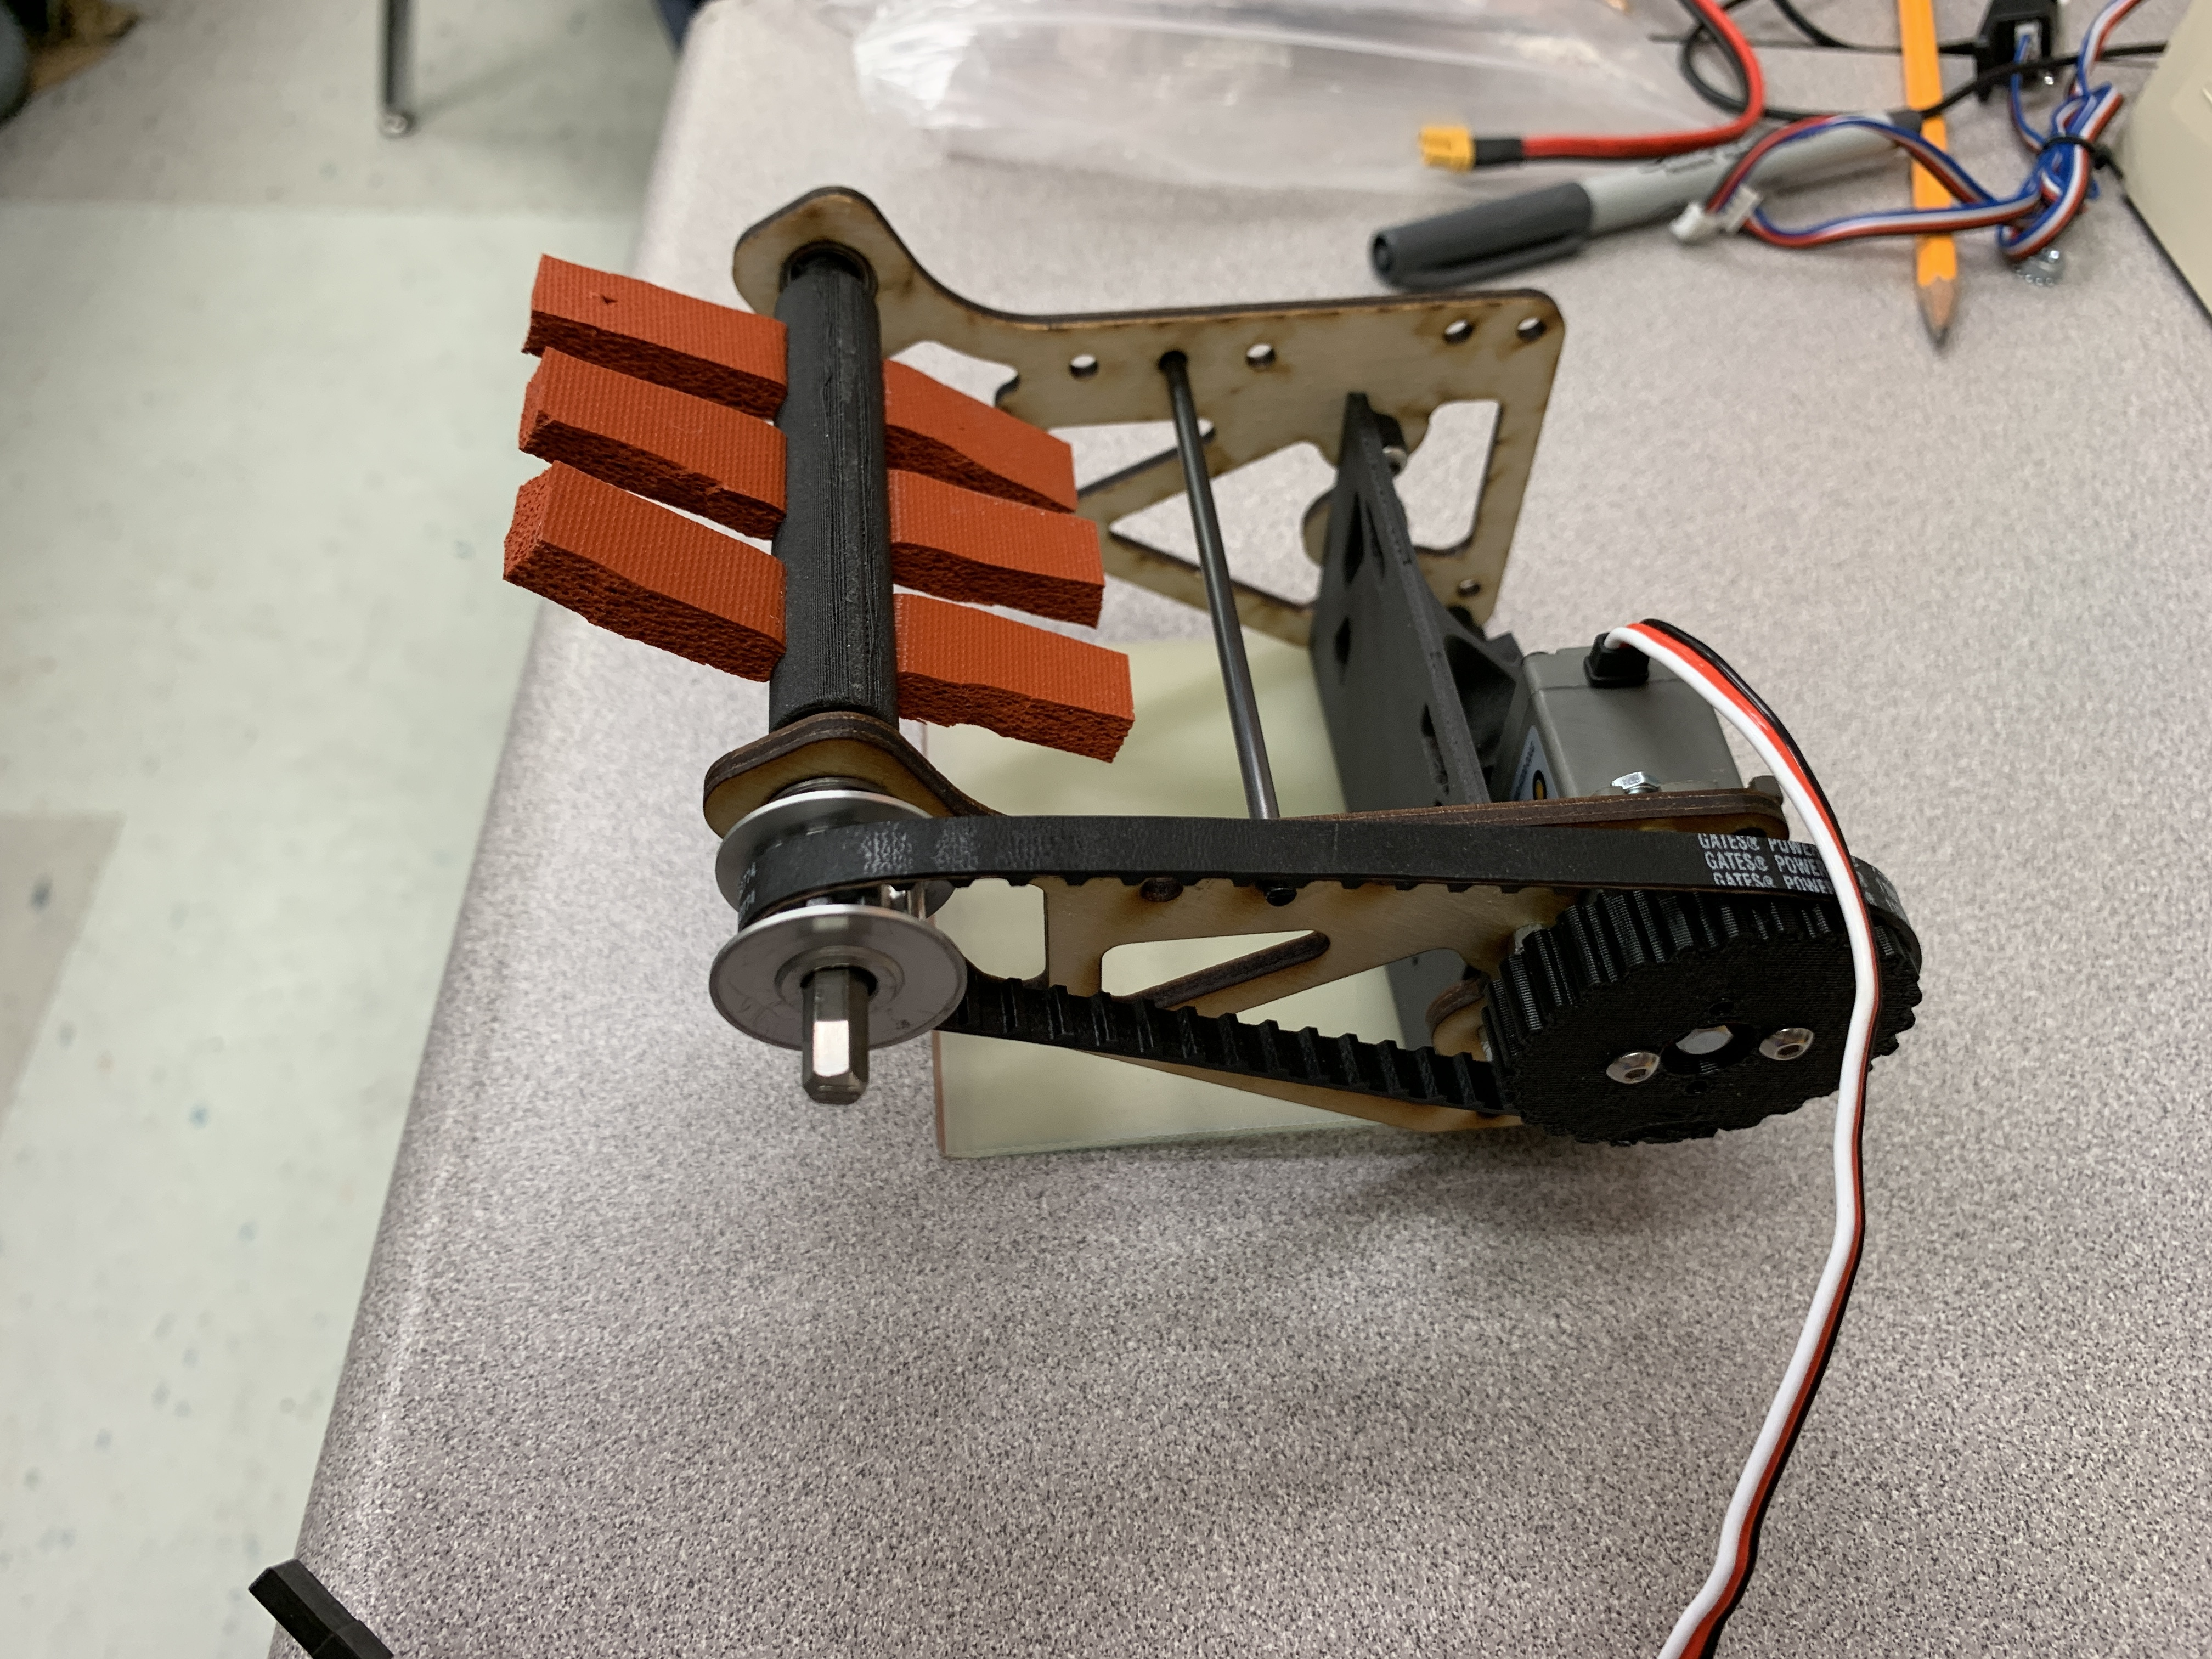
\includegraphics[width=0.95\textwidth, angle=0]{Meetings/January/01-11-22/1-11-22_Hardware_Figure1 - Nathan Forrer.JPG}
\caption{(Another) New intake}
\label{fig:pic3}
\end{figure}



\whatsnext{
\begin{itemize}
    \item Ensure that TricycleRRDrive works well with Road Runner before we begin to implement TRC event systems. 
    \item Give software time to finalize autonomous for upcoming meet
	\item Make any necessary adjustments to sweeper intake or other hardware

\end{itemize} 
}

